\documentclass[9pt]{beamer}
\usepackage{beamerpreamble}
\usepackage[swedish]{babel}
\usepackage{minted}
\usepackage{comment}
\usemintedstyle{vs}
\usepackage{xcolor}
\usepackage{tikz}
\usepackage{textgreek}
\usepackage{dirtytalk}
\usepackage{comment}

\renewcommand{\ttdefault}{cmtt}

\newcommand*\mean[1]{\bar{#1}}

\title{Datalaboration - Förberedande tutorial}
\author[benjamin.eriksson@physics.uu.se]{Benjamin Eriksson  \\ \tiny{med inspiration från} \\ \scriptsize{Slides av M. Isacson, M. Ellert, M. Olvegård, och B. Lindgren}}
\institute[Uppsala universitet]{{\small Avdelningen för tillämpad kärnfysik \\ Institutionen för fysik och astronomi} \\ \uulogo}
\date{{\small Reviderad}\\ \today}

\begin{document}

    \begin{frame}{Återkommande intervall}
        Efter denna föreläsning ska du kunna
        \begin{itemize}
            \item beräkna medelvärdet för ett återkommande intervall.
        \end{itemize}
    \end{frame}

    \begin{frame}
        \hrule \vspace{0.1cm}
        \textcolor{red}{Exempel:}
        Periodtiden för en pendel mäts genom att anteckna tiden $t_i$ vid varje fullbordad svängning.
        Detta ger mätserien $\{t_1, \ldots, t_i, \ldots, t_n\}$. Vi vill hitta medeltiden för en svängning.
        \vspace{0.1cm} \hrule
        
        \begin{block}{Fel approach}
            Det är lockande att ta medelvärdet genom
            \begin{equation*}
                \mean{t} = \frac{1}{n-1} \sum_i \Delta t_i = \frac{t_2 - t_1 + t_3 - t_2 + t_4 - t_3 + \ldots + t_n - t_{n-1}}{n - 1} = \frac{t_n - t_1}{n - 1}
        \end{equation*}
        \begin{itemize}
            \item hur många mätningar vi än gör används bara det första och sista mätvärdet!
        \end{itemize}
        \end{block}
       \vspace{0.2cm}
       \pause
       \begin{exampleblock}{Rätt approach}
            Använd metoden för återkommande intervall!
       \end{exampleblock}
       
    \end{frame}

    \begin{frame}{Återkommande intervall}
        \hrule \vspace{0.1cm}
        \textcolor{red}{Exempel:}
        Periodtiden för en pendel mäts genom att anteckna tiden $t_i$ för 6 fullbordade svängningar.
        Detta ger mätserien $t = [t_1, t_2, t_3, t_4, t_5, t_6]$. Vi vill hitta medeltiden för en svängning.
        \vspace{0.1cm} \hrule
        \vfill
        
        
        
        \onslide<+->
        Dela in mätningarna i en övre och undre halva och beräkna periodtiden mellan halvorna istället
        \begin{columns}
            \column{.6\textwidth}
            \begin{align*}
                T_1 &= \frac{t_4 - t_1}{3}\\
                T_2 &= \frac{t_5 - t_2}{3}\\
                T_3 &= \frac{t_6 - t_3}{3}\\
            \end{align*}
            \column{.4\textwidth}
            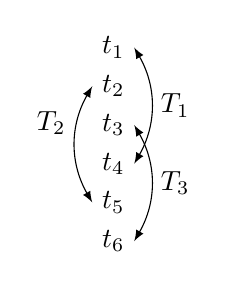
\begin{tikzpicture}
                \coordinate (dA) at (0,-1em);
                \coordinate (dB) at (0,-1.4em);
                \draw (0,0) node(t1){$t_1$}
                ++(dB)node(t2){$t_2$}
                ++(dB)node(tm){$t_3$}
                ++(dB)node(tm1){$t_4$}
                ++(dB)node(tm2){$t_5$}
                ++(dB)node(t2m){$t_6$};
                \draw[bend left,<->,>=latex] (t1.east) to node [auto] {$T_1$} (tm1.east);
                \draw[bend right,<->,>=latex] (t2.west) to node [auto,anchor=south east] {$T_2$} (tm2.west);
                \draw[bend left,<->,>=latex] (tm.east) to node [auto] {$T_3$} (t2m.east);
            \end{tikzpicture}
        \end{columns}
    Medelvärde och osäkerheter kan då beräknas med den nya mätserien 
    \begin{equation*}
        T = [T_1, T_2, T_3]    
    \end{equation*}
    
    \end{frame}

    \begin{frame}{Återkommande intervall}
        Obligatoriskt: 
        \begin{itemize}
            \item Öppna \textit{tutorial\_3.mlx} och gör sektionen \textcolor{orange}{Tutorial 3 - Återkommande intervall}.
            \item Svara på quizfrågorna i Studium.
        \end{itemize}
    \end{frame}

    \begin{frame}[fragile]
        I Matlab:
        \begin{minted}[frame=leftline,framesep=2mm,autogobble,escapeinside=||]{matlab}
        t = [1.06 2.01 2.98 3.96 5.02 6.02]; % mätdata |$t_i$|
        m = length(t)/2; % mittpunkten av mätserien |$m$|
        
        % övre och undre halvan av mätserien
        t_below = t(1:m);
        t_above = t(m+1:end);
        
        % frekvensen enligt formeln för återkommande intervall
        T = (t_above - t_below) / m;
        
        % medelvärdet och dess osäkerhetet beräknas som vanligt
        mT = mean(T);
        umT = std(T)/sqrt(m);
        \end{minted}

        \vfill
        Ovanstående exempel ger
        \begin{equation*}
            \mean{T} = \SI{0.994\pm0.014}{s} \quad \text{eller} \quad \mean{T} = 0.994\pm 0.014 \text{s}
        \end{equation*}
    \end{frame}

    \end{document}